\begin{figure}[ht]
\centerline{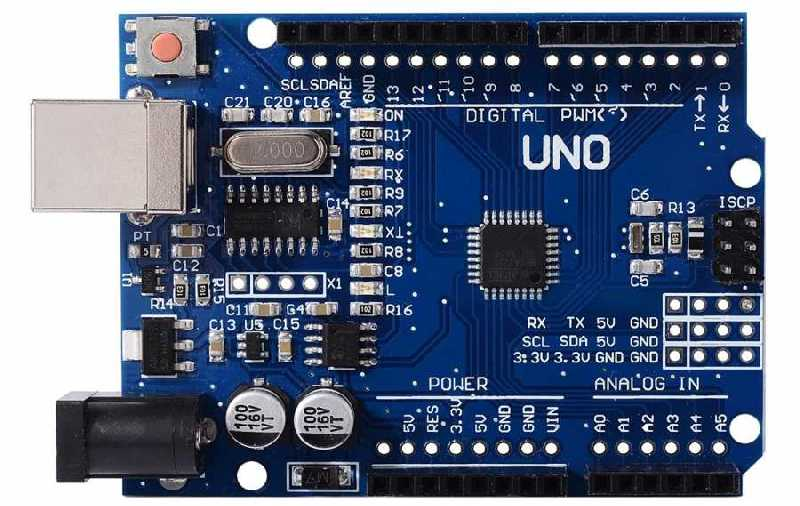
\includegraphics[width=0.4\textwidth]{figures/arduino.jpg}}
\caption{Gambar Arduino.}
\label{gmbr}
\end{figure}

\section{Cara menghubungkan arduino ke laptop}
Dalam artikel ini kami akan membahas cara menghubungkan arduino ke laptop\ref{gmbr}, untuk dapat memprogram Board Arduino, kita perlu software untuk melakukan programming dan menghubungkannya dengan PC. Langkah awalnya kita harus mendownload IDE arduino, kemudian instal aplikasi tersebut. Setelah di instal coba hubungkan arduino ke laptop, tunggu windows untuk melakukan driver instalation. Biasanya terjadi kegagalan.
Setelah arduino terhubung kita lanjutkan ke Langkah selanjutnya hubungkan arduino dengan PC menggunakan kabel usb yang tadi hingga PC mendeteksi arduino tersebut. Kemudian buka control panel windows,lalu buka device manager. Setelah itu cari ports (COM dan LPT), disana ada port port arduino UNO (COMxx), click kanan dan pilih "update driver software" option.
Lalu pilih "Browse my computer for driver software" option. Cari driver file dengan nama "arduino.inf", di folder drivers. Folder dapat ditemukan ditempat menginstal software IDE Arduino.
Setelah itu, dengan sendirina windows akan menyelesaikan instalasi driver. Kemudian sketch akan terbuka pada windows software Arduino anda,klik tipe board Arduino anda, karena anda menggunakan arduino uno, maka klik Arduino Uno.
Setelah memilih board yang sesuai dengan perangkat yang terhubung, maka selanjutnya anda harus memilih port yang menghubungkan PC dengan Arduino.
setelah program tersebut dapat terupload, di notifikasi akan muncul tanda atau pemberitahuan bahwa arduino sudah terhubung dengan laptop. Salah satu ciri arduino terhubung dengan laptop adalah LED 13 dari arduino akan berkedip-kedip selama 1 detik disetiap kedipannya.
setelah itu anda tinggal memasukkan kodingan agar arduino bekerja sesuai dengan kehendak anda.
Jika Prosedur diatas diikuti dengan baik dan benar maka arduino berjalan sesuai perintahnya.
Apabila terjadi masalah mengenai error menjalankan arduinonya berarti ada beberapa bug yang membuat Error ini terjadi.
Saat melakukan koding di Arduino pastikan tidak ada miss type atau typo dalam mengoding. Kesalahan sedikit akan membuat driver rusak dari kodingan itu sendiri
\section{Cara ke dua}
Selain cara di atas, ada juga cara lain menghubungkan arduino ke laptop.
\begin{enumerate}
\item Hubungkan kabel arduino dengan laptop
\item Buka device manager dengan cara klik kanan mycomputer
\item Klik other device jika arduino tidak muncul klik kanan dan update driver software kemudian pilih Browse my komputer for driver software kemudian pilih tempat arduino software disimpan.
\item Jika update software berhasil, klik tools di software arduino untuk pilih jenis board dan port yang dihubungkan dengan komputer.
\item Setelah dipilih, Siapkan koding sensor masing-masing kelompok.
\item Perhatikan Prosedur Kodingnya karena sedikit kesalahan akan terjadi kerusakan atau Error.
\item Jika Koding yang dikerjakan sudah teliti maka arduino siap untuk di
\end{enumerate}
\section{Arduino tidak terhubung}
Walaupun caranya mudah dan banyak tutorial langkah-langkahnya di youtube ataupun di google, tetapi tetap saja ada knedala saat menghubungkan arduino ke laptop, seringkali arduino tidak terbaca di laptop dan port tidak bisa dibuka dan muncul tulisan "uknown device" pada device manager.
Berikutnya saya akan menjelaskan bagaimana cara menangani situasi tersebut.
\begin{enumerate}
\item Klik kanan pada unknown device, pilih update driver siftware.
\item Setelah itu pilih browse my computer for driver software.
\item Pilih let me pick from a list from a list...
\item Pilih ports (COM\&LPT)
\item Klik next dan klik arduino LLC jika ada.
\item Jika belum ada klik have disk dan arahkan ke driver arduino yang sudah ada, pilih sesuai dengan boar arduino. setelah itu baru muncul arduino yang dimaksud.
\item Arduino akan succesfully dan terinstal / muncul pada com.
\item Arduino siap digunakan kembali.
\end{enumerate}